Já no teste de robustez a ruídos de medição dos controladores desenvolvidos, a Figura \ref{fig:graph_z_zdot_2kg_ruidos} mostra a resposta do sistema ao ruído de medição representado pela Figura \ref{fig:graph_sinal_ruidos}. A mesma resposta é mostrada na Figura \ref{fig:graph_z_zdot_2kg_details_ruidos}, porém com maiores detalhes, permitindo uma melhor comparação do sistema controlado pelos diferentes controladores.

Como se pode ver, o controlador neuro-\textit{fuzzy} obteve uma resposta melhor se comparado ao \textit{fuzzy}, apresentando uma redução em 39 \% na variação do sistema, além de uma convergência 13 \% mais rápida. Além disso, nota-se que, com o controlador neuro-\textit{fuzzy}, o sistema ficou mais estável, apresentando menores variações, apresentando assim, uma melhor resposta ao sistema sujeito a ruídos.

\begin{figure}[!htb]
    \centering
    \caption{Comparação da resposta das saídas $z$ e $\dot{z}$ no controle de altitude \textit{fuzzy} e neuro-\textit{fuzzy} para o sistema com massa $m=2$ kg sujeito a ruídos de medição da variável $z$}
    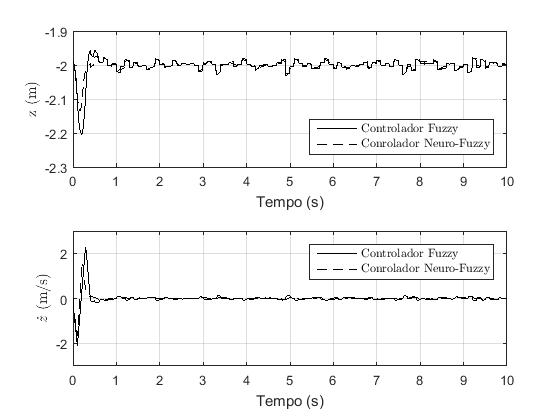
\includegraphics[width=1\textwidth]{./04-figuras/figuras_pos_banca/7-altitude2kg_ruido/graph_z_zdot_2kg_ruidos}
    \label{fig:graph_z_zdot_2kg_ruidos}
\end{figure}

\begin{figure}[!htb]
    \centering
    \caption{Sinal de ruído de medição sobre o valor real da variável $z$}
    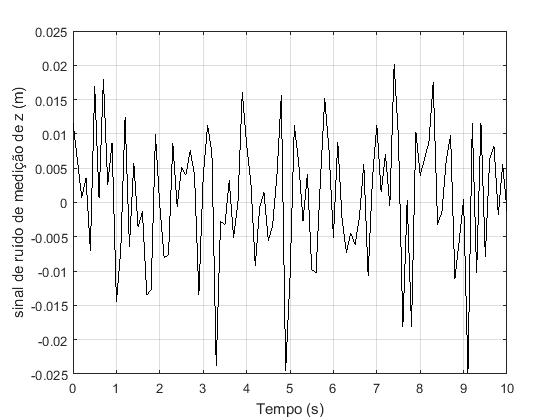
\includegraphics[width=0.7\textwidth]{./04-figuras/figuras_pos_banca/7-altitude2kg_ruido/graph_sinal_ruidos}
    \label{fig:graph_sinal_ruidos}
\end{figure}

\begin{figure}[!htb]
    \centering
    \caption{Comparação em mais detalhes da resposta das saídas $z$ e $\dot{z}$ no controle de altitude \textit{fuzzy} e neuro-\textit{fuzzy} para o sistema com massa $m=2$ kg sujeito a ruídos de medição da variável $z$}
    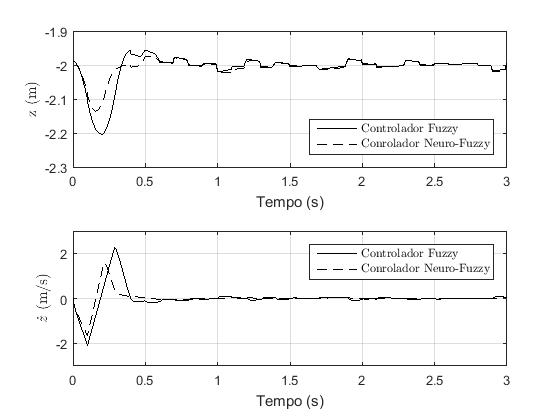
\includegraphics[width=1\textwidth]{./04-figuras/figuras_pos_banca/7-altitude2kg_ruido/graph_z_zdot_2kg_details_ruidos}
    \label{fig:graph_z_zdot_2kg_details_ruidos}
\end{figure}

Por fim, a Figura \ref{fig:graph_control_z_ruidos} mostra a resposta dos dois controladores ao longo tempo. Como se pode ver, o controlador neuro-\textit{fuzzy} apresentou eficiência energética 33 \% superior ao \textit{fuzzy} até o momento de convergência. Além disso, percebe-se que a ação do controlador neuro-\textit{fuzzy} é muito mais sutil na absorção dos ruídos, levando assim a um grande ganho de desempenho energético a longo prazo.

\begin{figure}[!htb]
    \centering
    \caption{Comparação da ação dos controladores \textit{fuzzy} e neuro-\textit{fuzzy} na estabilização em altitude do sistema com massa $m=2$ kg sujeito a ruídos de medição da variável $z$}
    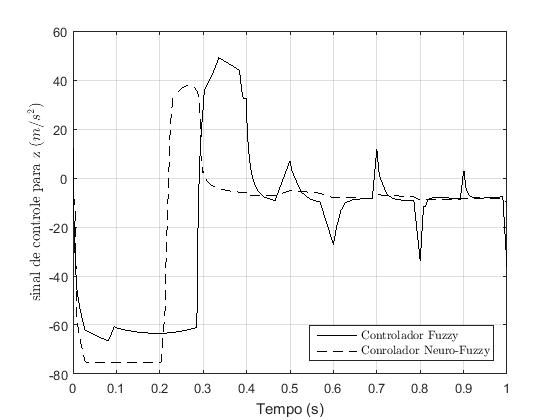
\includegraphics[width=0.6\textwidth]{./04-figuras/figuras_pos_banca/7-altitude2kg_ruido/graph_control_z_ruidos}
    \label{fig:graph_control_z_ruidos}
\end{figure}
